% !TEX encoding = UTF-8 Unicode
\documentclass[review]{elsarticle}

\usepackage{amsmath}
\usepackage{graphicx}
\usepackage{booktabs}
\usepackage{caption}
\usepackage{subcaption}
\usepackage{color, colortbl}
\definecolor{LightCyan}{rgb}{0.88,1,1}
% table position
\usepackage{float}
\restylefloat{table}

\usepackage{lineno,hyperref}

\modulolinenumbers[5]

\journal{Journal of \LaTeX\ Templates}

%%%%%%%%%%%%%%%%%%%%%%%
%% Elsevier bibliography styles
%%%%%%%%%%%%%%%%%%%%%%%
%% To change the style, put a % in front of the second line of the current style and
%% remove the % from the second line of the style you would like to use.
%%%%%%%%%%%%%%%%%%%%%%%

%% Numbered
%\bibliographystyle{model1-num-names}

%% Numbered without titles
%\bibliographystyle{model1a-num-names}

%% Harvard
%\bibliographystyle{model2-names.bst}\biboptions{authoryear}

%% Vancouver numbered
%\usepackage{numcompress}\bibliographystyle{model3-num-names}

%% Vancouver name/year
%\usepackage{numcompress}\bibliographystyle{model4-names}\biboptions{authoryear}

%% APA style
%\bibliographystyle{model5-names}\biboptions{authoryear}

%% AMA style
%\usepackage{numcompress}\bibliographystyle{model6-num-names}

%% `Elsevier LaTeX' style
\bibliographystyle{elsarticle-num}
%%%%%%%%%%%%%%%%%%%%%%%

\begin{document}

\begin{frontmatter}

\title{A-Track: A New Approach for Detection of Moving Objects in FITS Images}

%% Group authors per affiliation:

\author{T.~Atay}
\ead{atay@akdeniz.edu.tr}
\author{M.~Kaplan}
\author{Y.~Kilic}
\author{N.~Karapinar}

\address{Akdeniz University, Department of Space Sciences and Technologies, Antalya, Turkey}

\begin{abstract}
We have developed a fast, open-source, cross-platform pipeline, called A-Track, for detecting the moving objects (asteroids and comets) in sequential telescope images in FITS format. The pipeline is coded in Python 3. The moving objects are detected using an improved line detection algorithm, called ILDA. We tested the pipeline on astronomical data acquired by an SI-1100 CCD with a 
1-meter telescope. We found that A-Track performs very well in terms of detection efficiency, stability, and processing time. The code is hosted on GitHub under the GNU GPL v3 license.\\

\noindent
{\bf Program Summary:}

\noindent
{\em Program title: A-TRACK

\noindent
Catalogue identifier: 

\noindent
Program summary URL: https://github.com/akdeniz-uzay/A-Track

\noindent
Program obtainable from: https://github.com/akdeniz-uzay/A-Track

\noindent
Licensing provisions: Standard GNU General Public Licence version 3

\noindent
No. of lines in distributed program, including test data, etc.: 1040

\noindent
No. of bytes in distributed program, including test data, etc.: 34783

\noindent
Distribution format: .zip

\noindent
Programming language: Python 3

\noindent
Computer: Personal Computer

\noindent
Operating system: Any OS where Python 3 and subprograms are installed.

\noindent
Subprograms used: Numpy, Pandas, SExtractor, PyFITS, Alipy, f2n, docopt

}
\end{abstract}

\begin{keyword}
  line detection \sep minor planets \sep asteroids \sep image processing
  \MSC[2015] 10-13\sep  99-00
\end{keyword}

\end{frontmatter}

%\linenumbers

\section{INTRODUCTION}
Many research groups from all over the world contribute their best efforts to detect and track asteroids and comets. There are three main reasons behind this interest:
1) Asteroids and comets are the debris left over from the process that formed our solar system. Studying them gives us information about the formation of the solar system.
2) Our planet is hit by tons of particles everyday. Even though most of them are so small that they are destroyed in the atmosphere before they can reach the ground, the Tunguska meteor (60m) in 1908 \citep{Lyne1995} and the Chelyabinsk meteor (20m) in 2013 \citep{Popova1069} remind us that relatively large objects do strike the Earth and cause significant damage occasionally. Such potentially dangerous objects should be carefully studied to understand their sizes and trajectories.
3) Asteroids and comets offer a rich supply of minerals and raw materials. We can benefit from studying their compositions and structures.

Most of the research groups that study asteroids and comets use robotized telescopes with high-resolution cameras and optical systems to scan the sky all night long. However, to our best knowledge, none of these groups use an open-source/free software that detects asteroids and comets automatically.

In this work, we introduce a new Improved Line Detection Algorithm for the detection of celestial moving objects, called ILDA. The idea comes from Chen's Randomized Line Detection (RLD) algorithm \citep{chen2001}. We modified and improved RLD to make it applicable to sequential telescope images in FITS format. Our algorithm needs at least 3 sequential images of the same sky region taken one after the other. Even though the images don't have to be taken on the same night, the duration of the observation should not be too long as an object to be detected can leave the region.

We used ILDA to develop an open-source (licensed under GPL v3), cross-platform pipeline called A-Track. It is easy to use and fast. It doesn't need human interaction while running. The coding was done in Python 3 as it is easy to understand and has many astronomical modules to work with. It will run on any operating system where Python 3 and the dependencies are installed. We tested A-Track on GNU/Linux (Fedora 20, Ubuntu 14.04) and Mac OS X (10.10.4, Yosemite) without any problems.

The workflow of the pipeline, the packages used, and details about the developing stage are given in sections 2, 3, and 4. In section 5, we present some test results, moving objects detected by A-Track on two data sets.


\section{A-TRACK: OVERVIEW} %\label{sec:detection}

In principle, the moving objects in sequential CCD images can be identified by tracking their motion with respect to the stationary objects (stars). One requirement is that the moving object is detected by the telescope/CCD system in most (if not all) of the images. Another requirement is that the moving object is fast enough that its motion from image to image is detectable. Our algorithm is based on the idea that, over short enough intervals of observation time (which can be days or even weeks depending on the position and speed of the object) the trajectory of a moving celestial object can be approximated by a line segment.

The workflow of A-Track is shown in Fig.~\ref{fig:workflow}. The program consists of five main files: atrack.py, sources.py, asteroids.py, visuals.py, and atrack.config. atrack.py is the main file to be executed with Python 3 via the command-line. On any OS where all dependencies are installed, it can be invoked with

\begin{verbatim}
python3 atrack.py <fits_dir> [--ref=<ref_image>]
                             [--skip-align] [--skip-cats] 
                             [--skip-pngs] [--skip-gif]
\end{verbatim}

\verb;<fits_dir>; is the path of the directory where the telescope images to be analyzed are located. Unless the \verb;--ref=<ref_image>; option is used, the first image file in lexicographical order is used as the reference image for alignment. The rest of the options will be discussed in the following sections.

\begin{figure}[!h]
  \centering
  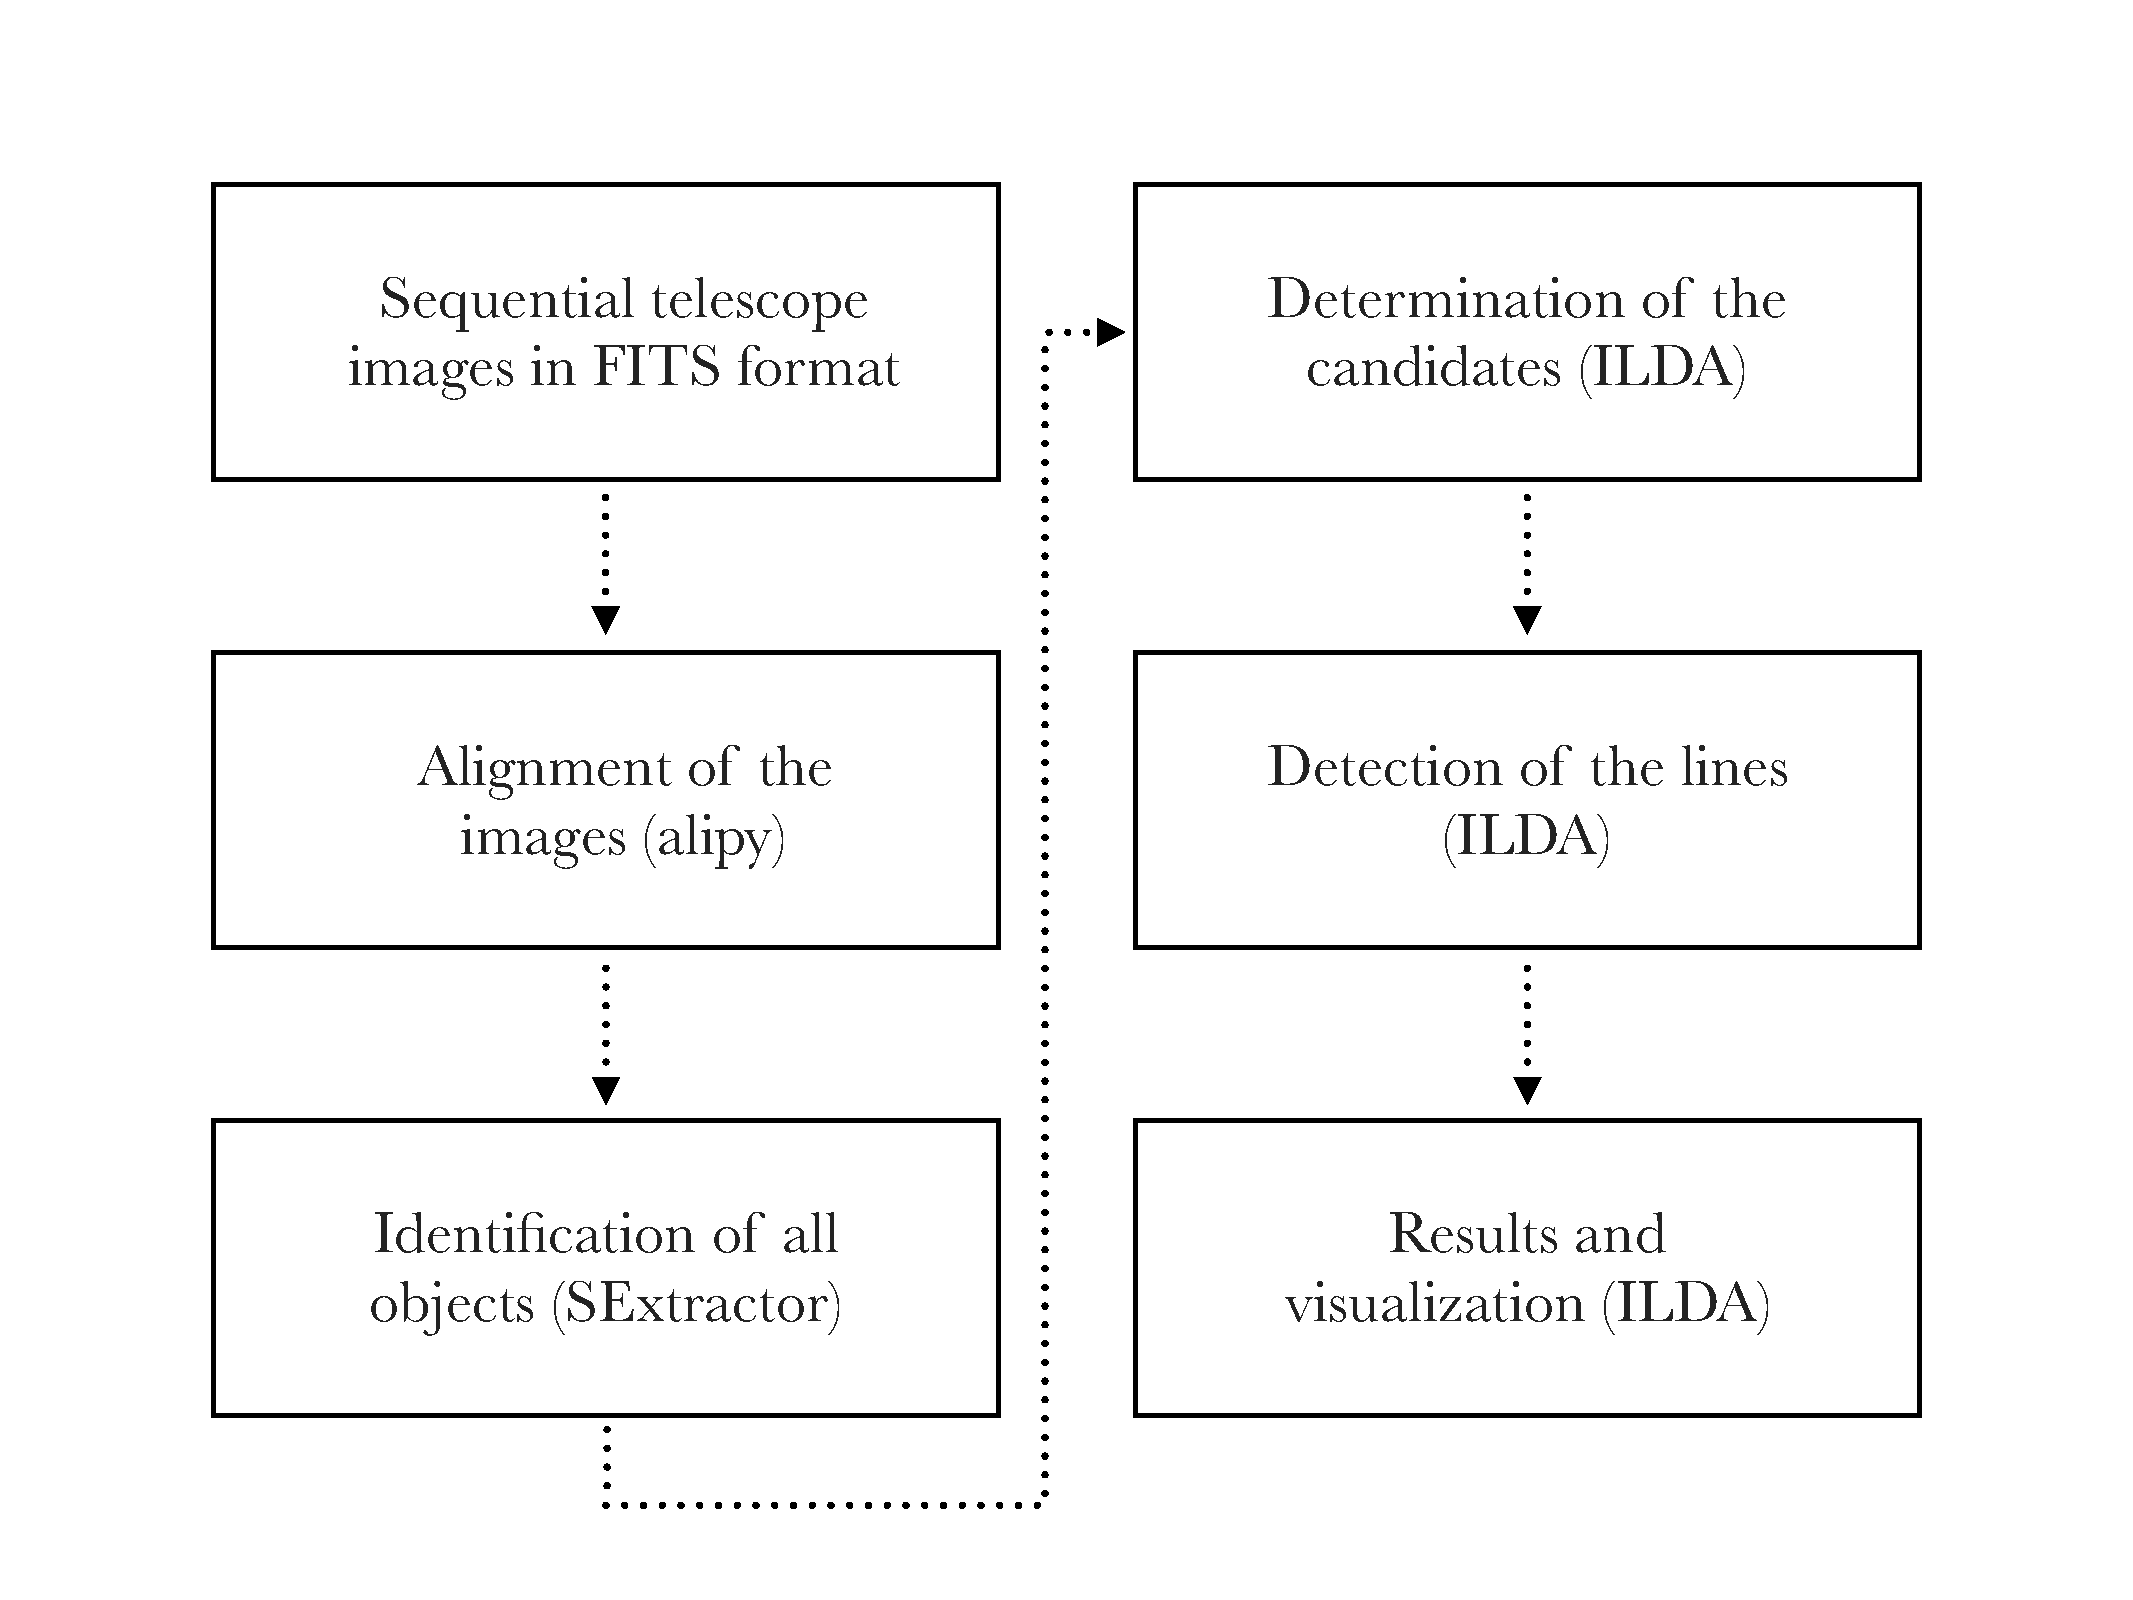
\includegraphics[width=1.0\textwidth]{figure_1_workflow}
  \caption{A-Track workflow.}
  \label{fig:workflow}
\end{figure}


sources.py, asteroids.py, and visuals.py are the three modules imported by atrack.py to handle the alignment of the images, the identification of the objects, the detection of the moving objects, and the visual outputs. Usually, the detection of the moving objects is the most CPU-demanding step. Therefore, to reduce the processing time, ILDA was coded using the parallel processing architecture in Python 3.

All of the parameters explicitly used by A-Track can be found, together with their descriptions, in the configuration file atrack.config. Some of the default parameters in this file are specific to the telescope/CCD system used, while the rest of them are purely empirical. The user is expected to use the parameter values appropriate for his/her own images.

All of the FITS images in \verb;<fits_dir>; are used for detection. Also, unless it already exists, a directory named atrack is created in \verb;<fits_dir>; where all outputs from A-Track for that particular image set are saved.

\section{IMAGES, ALIGNMENT, and OBJECT IDENTIFICATION} %\label{conclusion}

There are a few requirements for the images to be analyzed by A-Track: They need to be in FITS format. The FITS-headers need to comply with the FITS standarts \citep{fits_standarts} as the key parameters DATE-OBS, EXPTIME, XBIN, YBIN, NAXIS1, and NAXIS2 are explicitly used by ILDA. A-Track needs at least 3 sequential FITS images to run. Usually, 5 to 10 images are enough to detect all of the detectable (limited by the image quality) moving objects in the images. A-Track can work with raw images (no pre-reduction is needed). It assumes the images are lexicographically ordered in time. The x and y binnings of the images need to be the same. The parameters in the [sources] section of the configuration file are used for alignment and identification.

To align the images, A-Track uses the Python module alipy \citep{alipy}, selecting one of the images as the reference. alipy first determines the affine transformation matrices between the images and the reference,  following Lang's method \citep{lang2010}. It then uses the affine transform function of the scipy module to align all of the images with respect to the reference. The aligned images are saved in the atrack/ directory in FITS format with the suffix `\_affineremap'. If the images to work with are already aligned, this process can be skipped using the \verb;--skip-align; option in the command-line interface.

A-Track uses the latest stable version 2.19.5 of SExtractor to identify the (light) sources in the CCD images. It is invoked via the pysex submodule (wrapper) in alipy. The default values for the user-defined parameters used in the identification process can be found in the [sources] section of the configuration file. For each image, a catalog file with the extension .pysexcat is created in the atrack/ directory. This catalog file contains the internal flags (FLAGS), the x and y coordinates (X\_IMAGE, Y\_IMAGE), the flux and its RMS error (FLUX\_AUTO, FLUXERR\_AUTO), the local sky background (BACKGROUND), the FWHM (FWHM\_IMAGE), and the elongation (ELONGATION) for each object identified by SExtractor in that particular image \citep{bertin1996}. If the objects in the images are already identified, this process can be skipped using the \verb;--skip-cats; option in the command-line interface.

Once all of the objects in all of the images are identified, that is, a catalog file is created for each image, A-Track treats the objects as points for the purpose of moving object detection, with coordinates given in the respective catalog file. Therefore, we will use the words `object' and `point' interchangeably in the rest of the paper.

\section{MOVING OBJECT DETECTION}

\subsection{Elimination of Stationary Objects}

The first step in moving object detection is to eliminate the objects that are clearly stationary from the catalogs so that one is left with the moving object candidates for further analysis. The elimination process is based on the user-defined parameters in the [asteroids] section of the configuration file. In addition to truly moving objects, these candidates may contain cosmic rays as well as objects that appear to move due to atmospheric seeing or pixel saturation. Once the candidates are determined for each image, the internal flags (FLAGS), the x and y coordinates (X\_IMAGE, Y\_IMAGE), the flux (FLUX\_AUTO), and the local sky background (BACKGROUND) values for these candidates are saved in the atrack/ directory as a file with the extension .cnd.

To decide whether or not an object is a candidate, A-Track performs several checks. The FLAGS value of a candidate cannot be greater than FLAG\_MAX in the configuration file. The default value 31 of FLAG\_MAX ensures that the objects with bright and close neighbors, the objects blended with another object, the objects with saturated pixels, and the objects close to or on the image boundary are not discarded during the identification. The FWHM of a candidate cannot be smaller than FWHM\_MIN defined in the configuration file. The user can set the maximum FWHM via the FWHM\_COEFFICIENT parameter in the configuration file (the default value is 2.5). A candidate object's FWHM cannot be greater than FWHM\_COEFFICIENT times the average FWHM of all identified objects. The FLUX\_AUTO value of a candidate has to be between BACKGROUND and FLUX\_MAX, both of which are defined in the configuration file. The FLUX\_AUTO/FLUXERR\_AUTO ratio of a candidate cannot be smaller than SNR\_MIN defined in the configuration file. The ELONGATION value of a candidate cannot be greater than ELONGATION\_MAX defined in the configuration file.

To perform the final check, first, the catalog files generated by SExtractor are merged into one large catalog file called master.pysexcat, which is also saved in the atrack/ directory. Then, A-Track checks if the object has the same x and y coordinates (within a tolerance of TRAVEL\_MIN defined in the configuration file) in more than one image. To do this, it calculates the distances, one by one, between the object and all of the objects in the master catalog file. To determine the number of occurrences where the calculated distance is less than TRAVEL\_MIN, it uses the logic equation

\begin{equation}
 N = \sum_{\begin{smallmatrix}\scriptsize \mbox{all objects}  \end{smallmatrix}} \left( \sqrt{\left( \left( C_x - O_x \right) ^ 2 + \left( C_y - O_y \right) ^ 2 \right)} \leq TRAVEL\_MIN \right)
\end{equation}
\\
\noindent
where $N$ is the number of occurrences, $C$ is the candidate being investigated, $O$ is the object in the master.pysexcat file that is being compared, and the subscripts $x$ and $y$ denote the $x$ and $y$ coordinates, respectively. The result of the summand is 1 if the inequality holds, 0 otherwise. If $N$ is found to be 1 for the object, then the object is tagged as a candidate.

\subsection{ILDA: An Improved Line Detection Algorithm}

Once the candidates are found for each image (catalog file), ILDA looks for points from different images that would form a line when plotted on the same graph. This is explained in Fig.~\ref{fig:objects}. The lines ILDA seeks will not be on any particular image, but rather form when all points in all images are plotted on the same graph. Each object on any of these lines will belong to a different image.

\begin{figure}[!h]
  \centering
  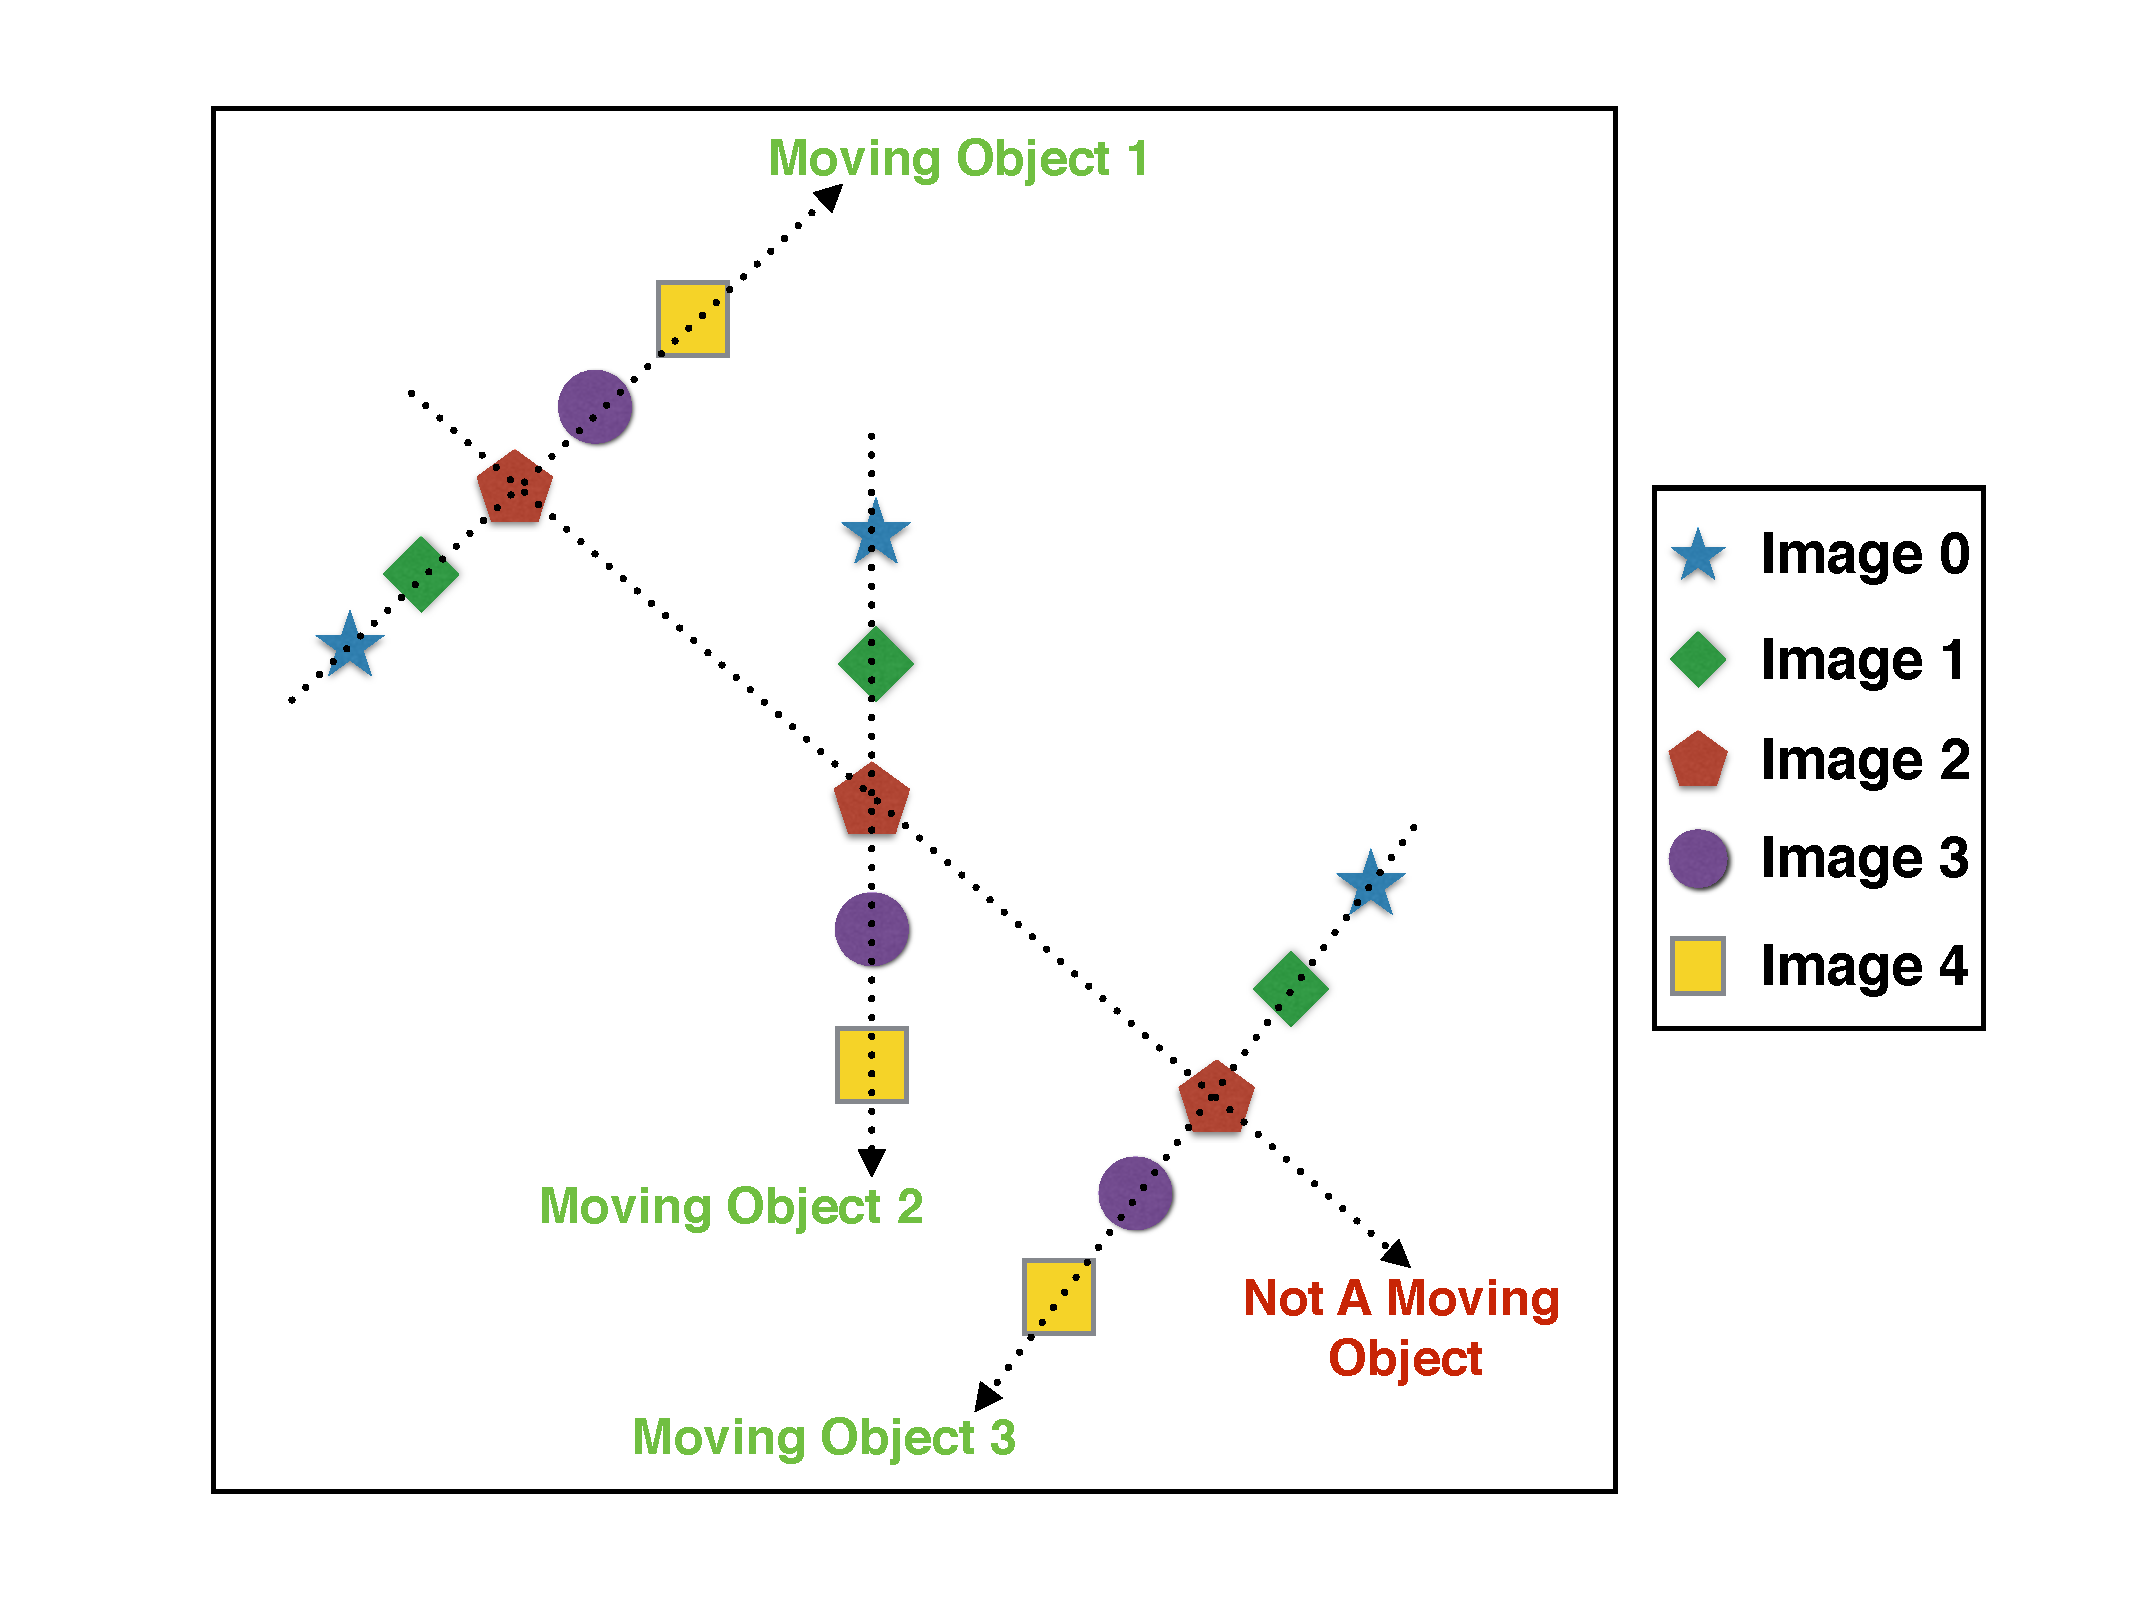
\includegraphics[width=1.0\textwidth]{figure_2_objects}
  \caption{Lines sought by ILDA to determine the moving objects. Lines formed by points on different images are accepted. Lines formed by points on the same image are rejected.}
  \label{fig:objects}
\end{figure}

In addition to this forming-a-line requirement, ILDA also applies some time constraints that will be explained below. That is, forming a line is not enough for those objects to be considered as moving objects. They need to be at the right positions on that line. The time information (observation time and exposure time) of the images are read from the FITS-headers. The observation times need to be in \verb;%Y-%m-%dT%H:%M:%S.%f; or \verb;%Y-%m-%dT%H:%M:%S; format. The parameters in the [asteroids] section of the configuration file are used for line detection.

The first step of ILDA is to find all of the 3-point segments that would belong to a kind of line described above. To do this, ILDA investigates all of the possible 3-point combinations obtained from all of the candidate files (.cnd), each point coming from a different image. The points in these combinations are ordered as 1, 2, and 3 according to the observation times of the corresponding images. For each 3-point combination, it performs three checks.

First, it looks at the first two points to perform a distance check. It demands that the distance between these two points is smaller than $d_{max}$ given by

\begin{equation}
        d_{max} = \left( OT_2 - OT_1 + \frac {ET_2 - ET_1} {2} \right) \cdot \frac {V\_MAX} {SCALE \cdot XBIN}
\end{equation}
\\
\noindent
where $OT$ is the observation time, $ET$ is the exposure time, V\_MAX and SCALE are the maximum angular velocity of the sought object and the pixel scale subtended by the telescope/CCD system, respectively, defined in the configuration file, XBIN is the x-binning of the image the first point belongs to (read from the FITS-header), and the subscripts 1 and 2 denote the first and the second points, respectively. If the distance between the first two points of a 3-point combination is not smaller than $d_{max}$, ILDA eliminates that 3-point combination.

If a 3-point combination passes the distance check, then ILDA performs a speed check. As shown in Fig.~\ref{fig:velocity}, the speed of the object between points 1 and 2 need to be approximately equal to the speed between points 2 and 3. The approximity is controlled by the TOLERANCE parameter defined in the configuration file. ILDA demands that the following inequality is satisfied

\begin{equation}
        \left | {d_{23} - \frac {d_{12}}{t_{12}} \cdot t_{23}} \right | \leq TOLERANCE
\end{equation}
\\
\noindent
where $d_{ij}$ and $t_{ij}$ are the distance and the time, respectively, between points $i$ and $j$.

\begin{figure}[!h]
  \centering
  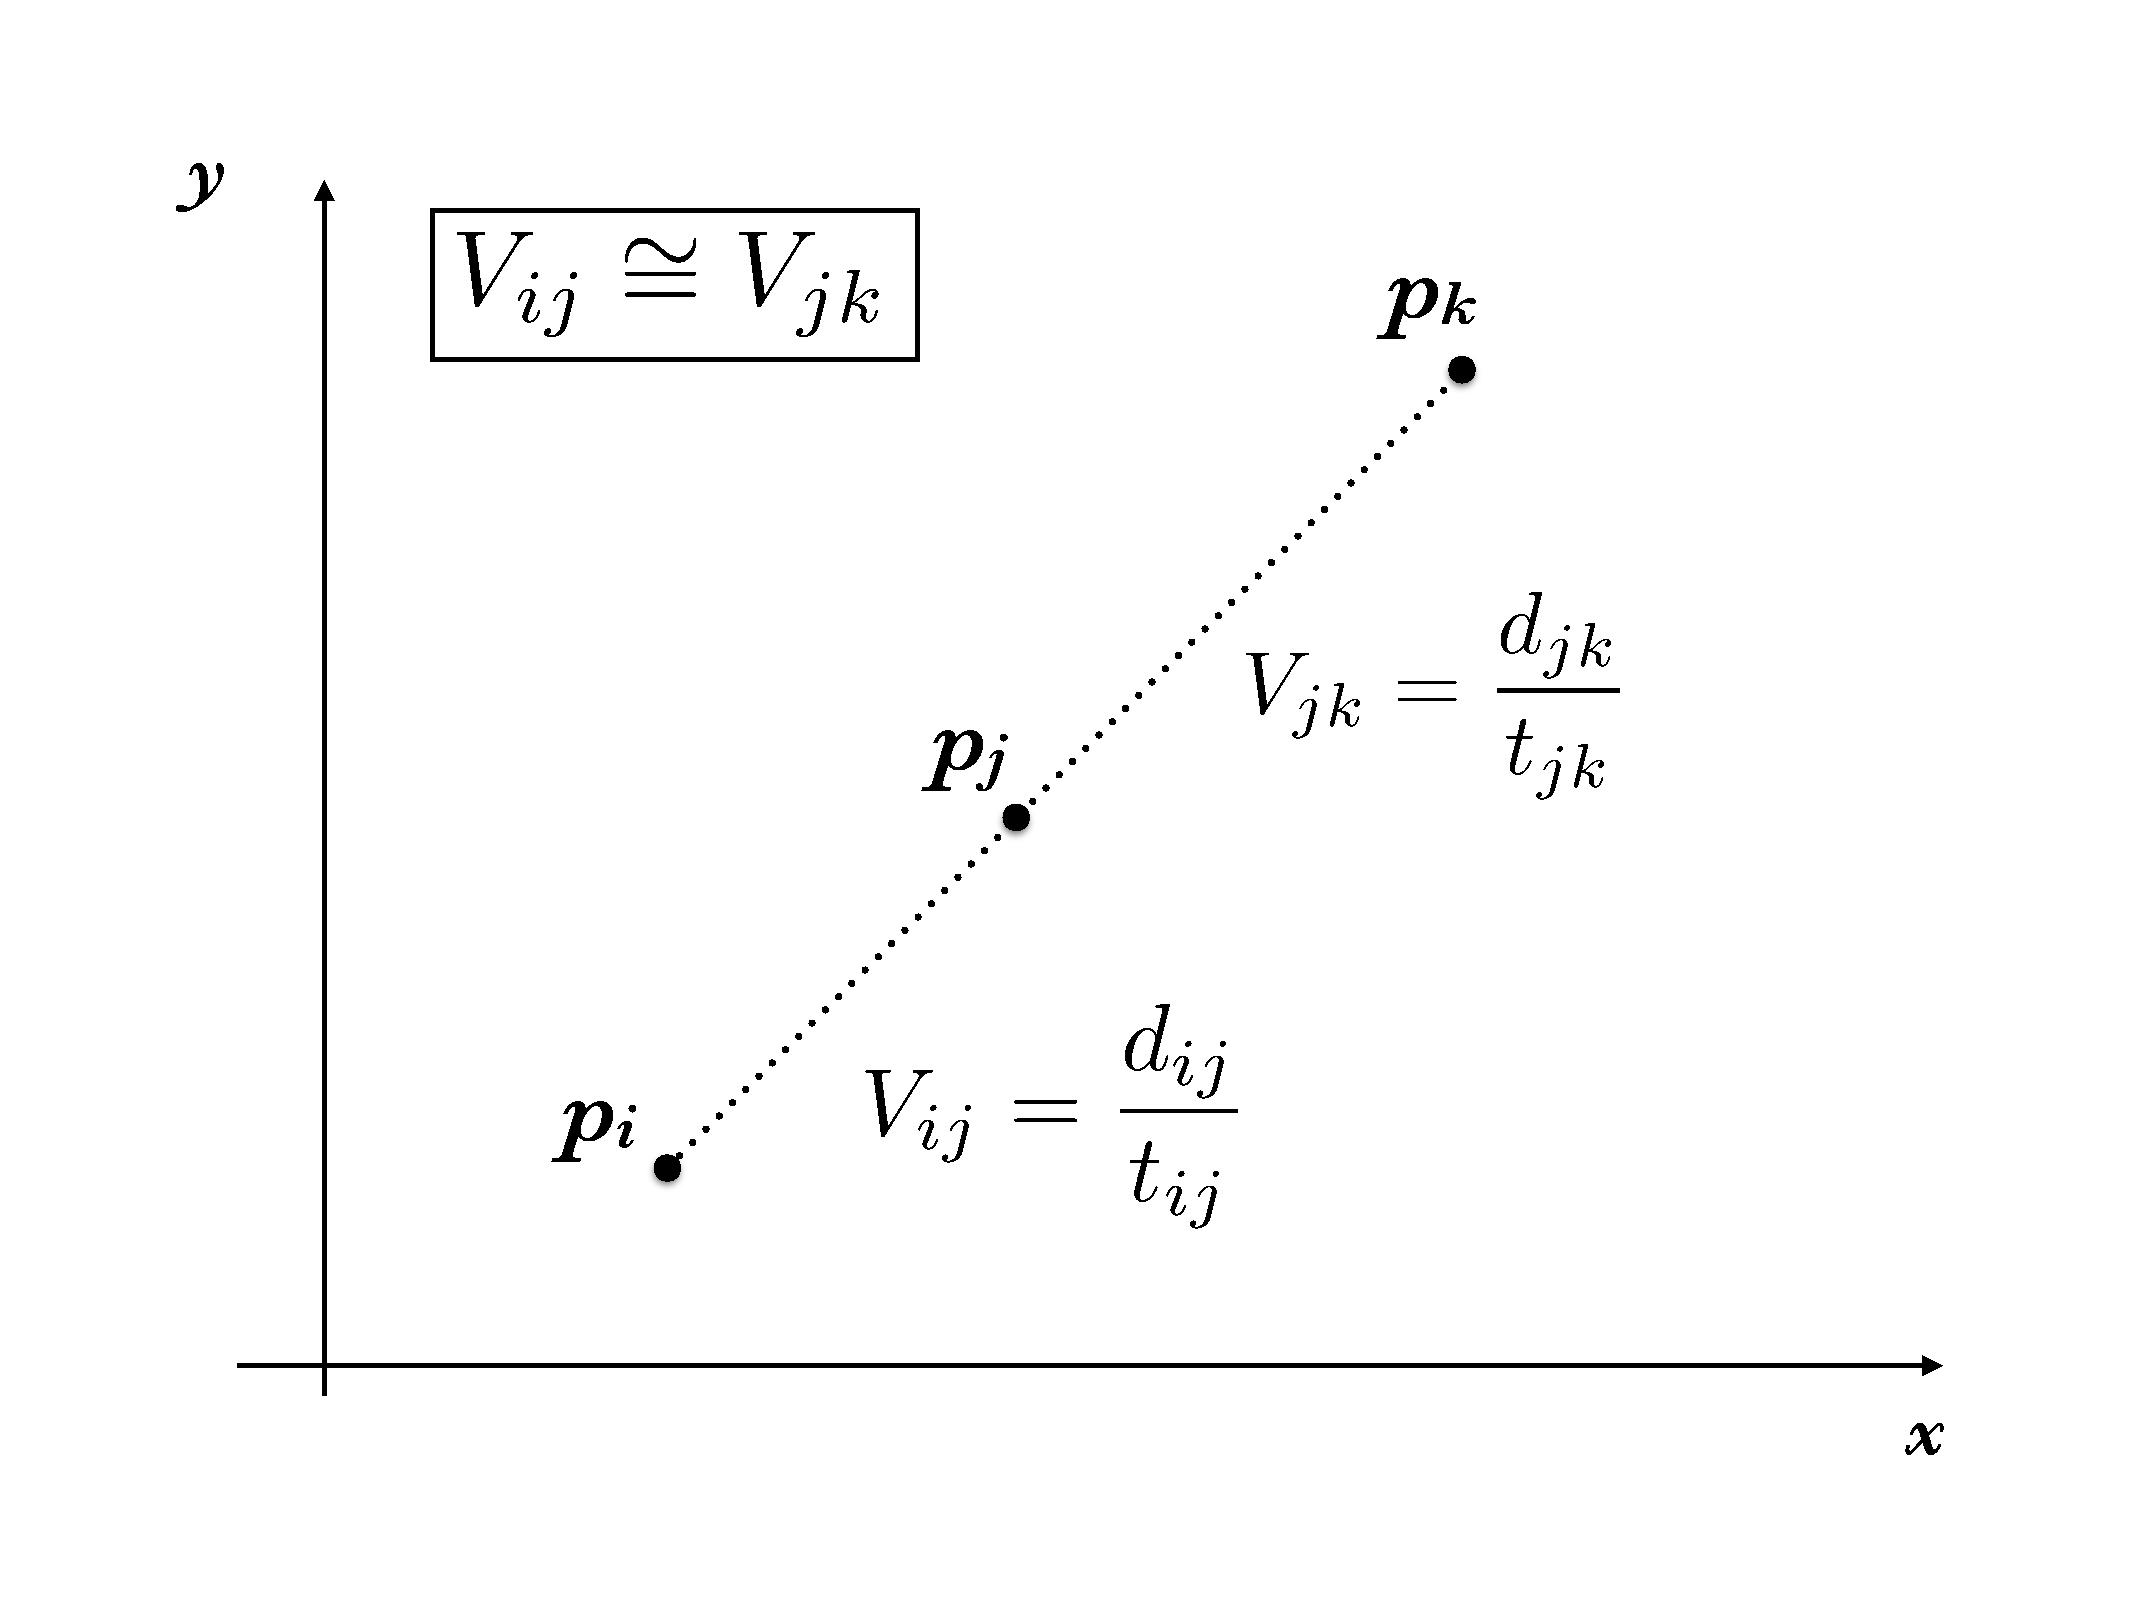
\includegraphics[width=1.0\textwidth]{figure_3_velocity}
  \caption{Speed check performed by ILDA to determine the moving objects. For points $p_i$, $p_j$, and $p_k$ in a 3-point combination, the speed between points $i$ and $j$ need to be approximately equal to the speed between points $j$ and $k$.}
  \label{fig:velocity}
\end{figure}

If a 3-point combination passes both checks (distance and speed), then ILDA performs a final check, collinearity. Considering the triangle formed by these 3 points, ILDA demands that the length of the longest side of this triangle is greater than 2 $\times$ TRAVEL\_MIN and the height associated with this side is smaller than HEIGHT\_MAX, as shown in Fig.~\ref{fig:linesegment}. Both of these parameters are defined in the configuration file.

\begin{figure}[!h]
  \centering
  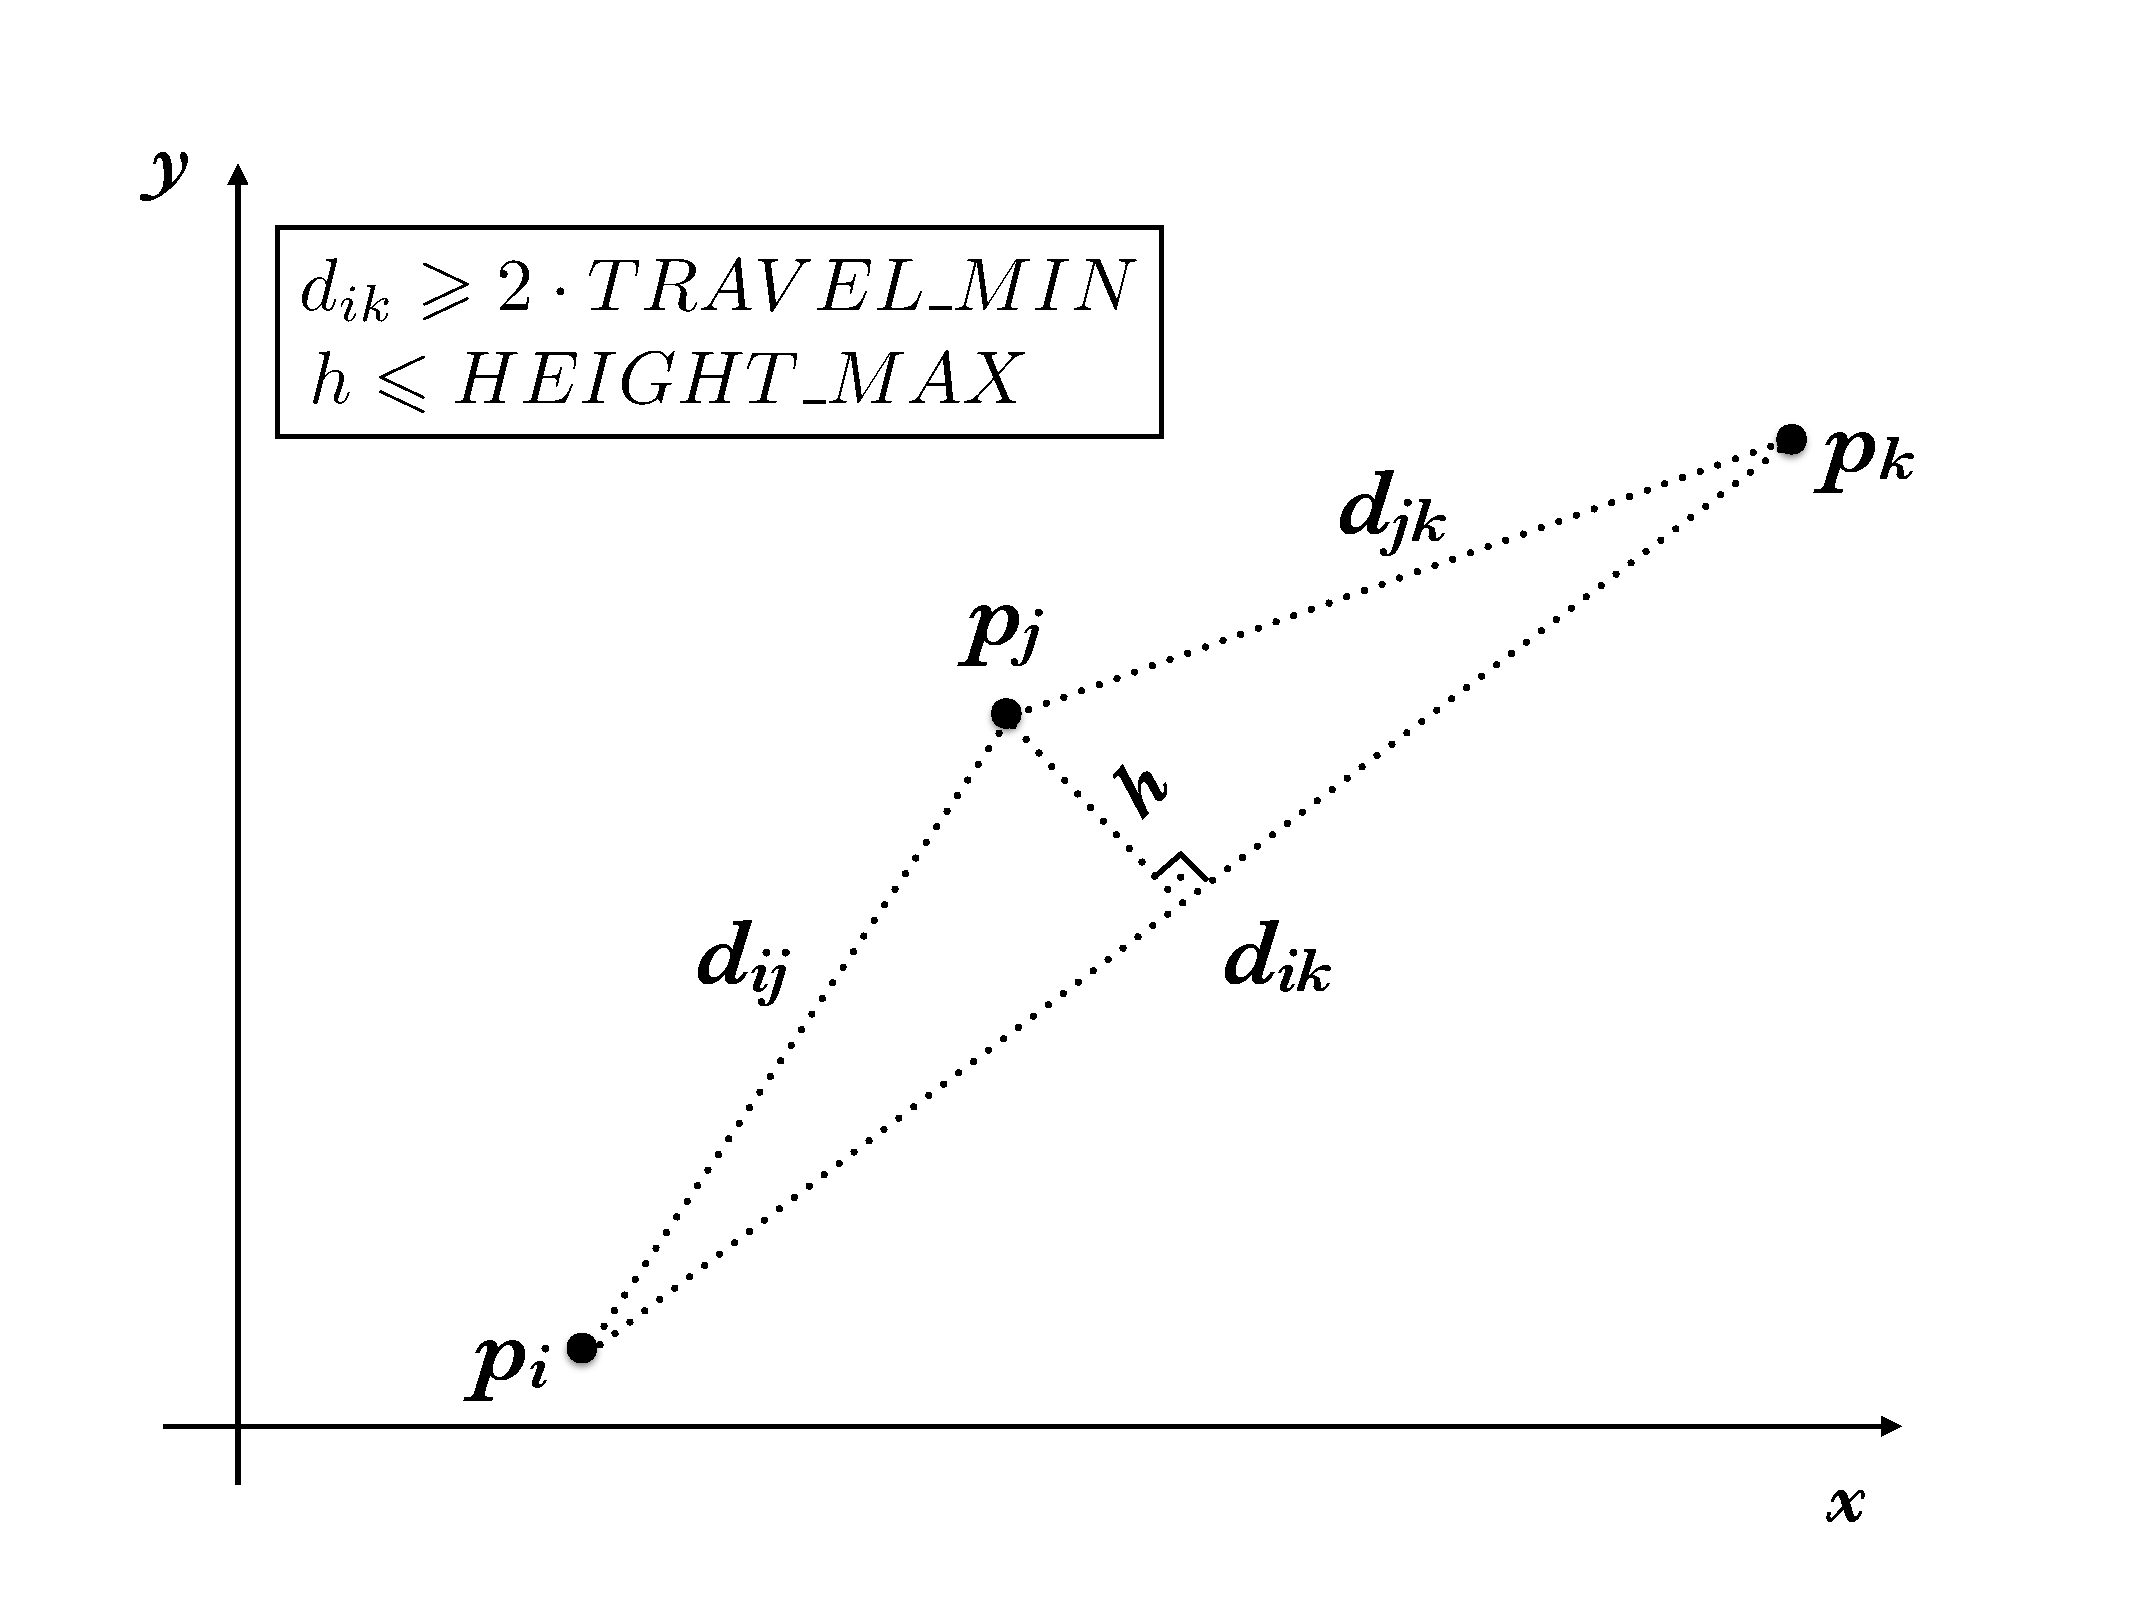
\includegraphics[width=1.0\textwidth]{figure_4_line_segment}
  \caption{Collinearity check performed by ILDA to determine the moving objects. A triangle is formed by points $p_i$, $p_j$, and $p_k$ of a 3-point combination. If the length of the longest side of this triangle is $d_{ik}$ and the height associated with this side is $h$, then ILDA demands that $d_{ik} \geq 2 \cdot TRAVEL\_MIN$ and $h \leq HEIGHT\_MAX$.}
  \label{fig:linesegment}
\end{figure}

Once ILDA determines all of the 3-point segments that pass the distance, the speed, and the collinearity criteria, it merges the segments that belong to the same line. In the end, there will be as many lines as the number of moving objects in the images. Each line, hence each moving object, is assigned an ID number called ObjectID (starting from 1). The detected objects are divided into two groups: moving objects and uncertain objects. If the speed of a detected object is greater than SPEED\_MIN defined in the configuration file, then it is classified as moving. Otherwise, it is classified as uncertain. The default value for SPEED\_MIN is 0.1 (pixels/min). The detected objects with speeds smaller than this value are usually not moving objects but artifacts. ILDA leaves the decision to the user.

The detected moving objects are printed on the screen and saved in the results.txt file in atrack/ directory. The first few lines of a sample results.txt file are shown in Fig.~\ref{fig:results}. Each point on a detected line is included in the result. ObjectID is the ID number of the object (line) the point belongs to. Hence, the highest ObjectID is the number of different moving objects detected in the images. FileID is the number of the image file the point belongs to (the image files are numbered in lexicographical order, starting from 0). Flags is the internal flags code generated by SExtractor for that particular point. x and y values are the x and y coordinates of the point in the (aligned) image it belongs to. Flux, Background, and Speed values for the point are also included in the result.

\begin{figure}[!h]
  \centering
  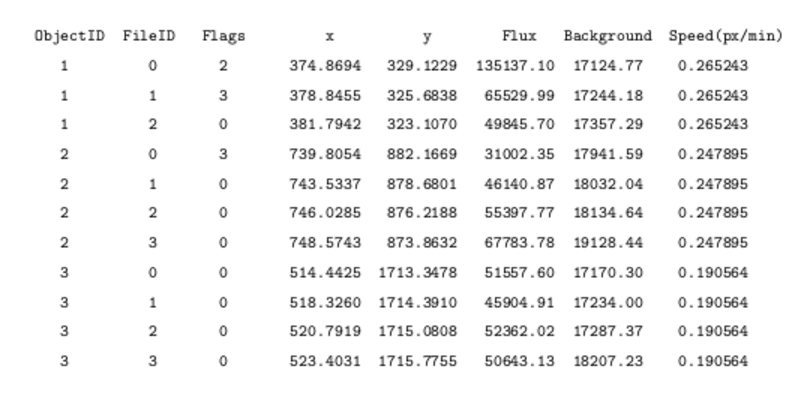
\includegraphics[width=1.0\textwidth]{figure_5_results_file}
  \caption{First few lines of a sample results.txt file. Different objects have different ObjectIDs. FileID gives the lexicographical order of the image file a particular point belongs to.}
  \label{fig:results}
\end{figure}

\subsection{Visualization}

Once the detection of moving objects is complete, the user can check the results in visual form as well. The only parameter used for visualization is SPEED\_MIN in the [visuals] section of the configuration file. Using the f2n module, A-Track converts each aligned image into PNG format, encircling the moving and the uncertain objects on the image. For each aligned image, a file is created in the atrack/ directory with the extension .png. As seen in Fig.~\ref{fig:realimage}, green and red circles are used to mark the moving and the uncertain objects, respectively, and the ObjectID associated with the object is printed next to the circle. The PNG conversion can be skipped using the \verb;--skip-pngs; option in the command-line interface.

\begin{figure}[!h]
  \centering
  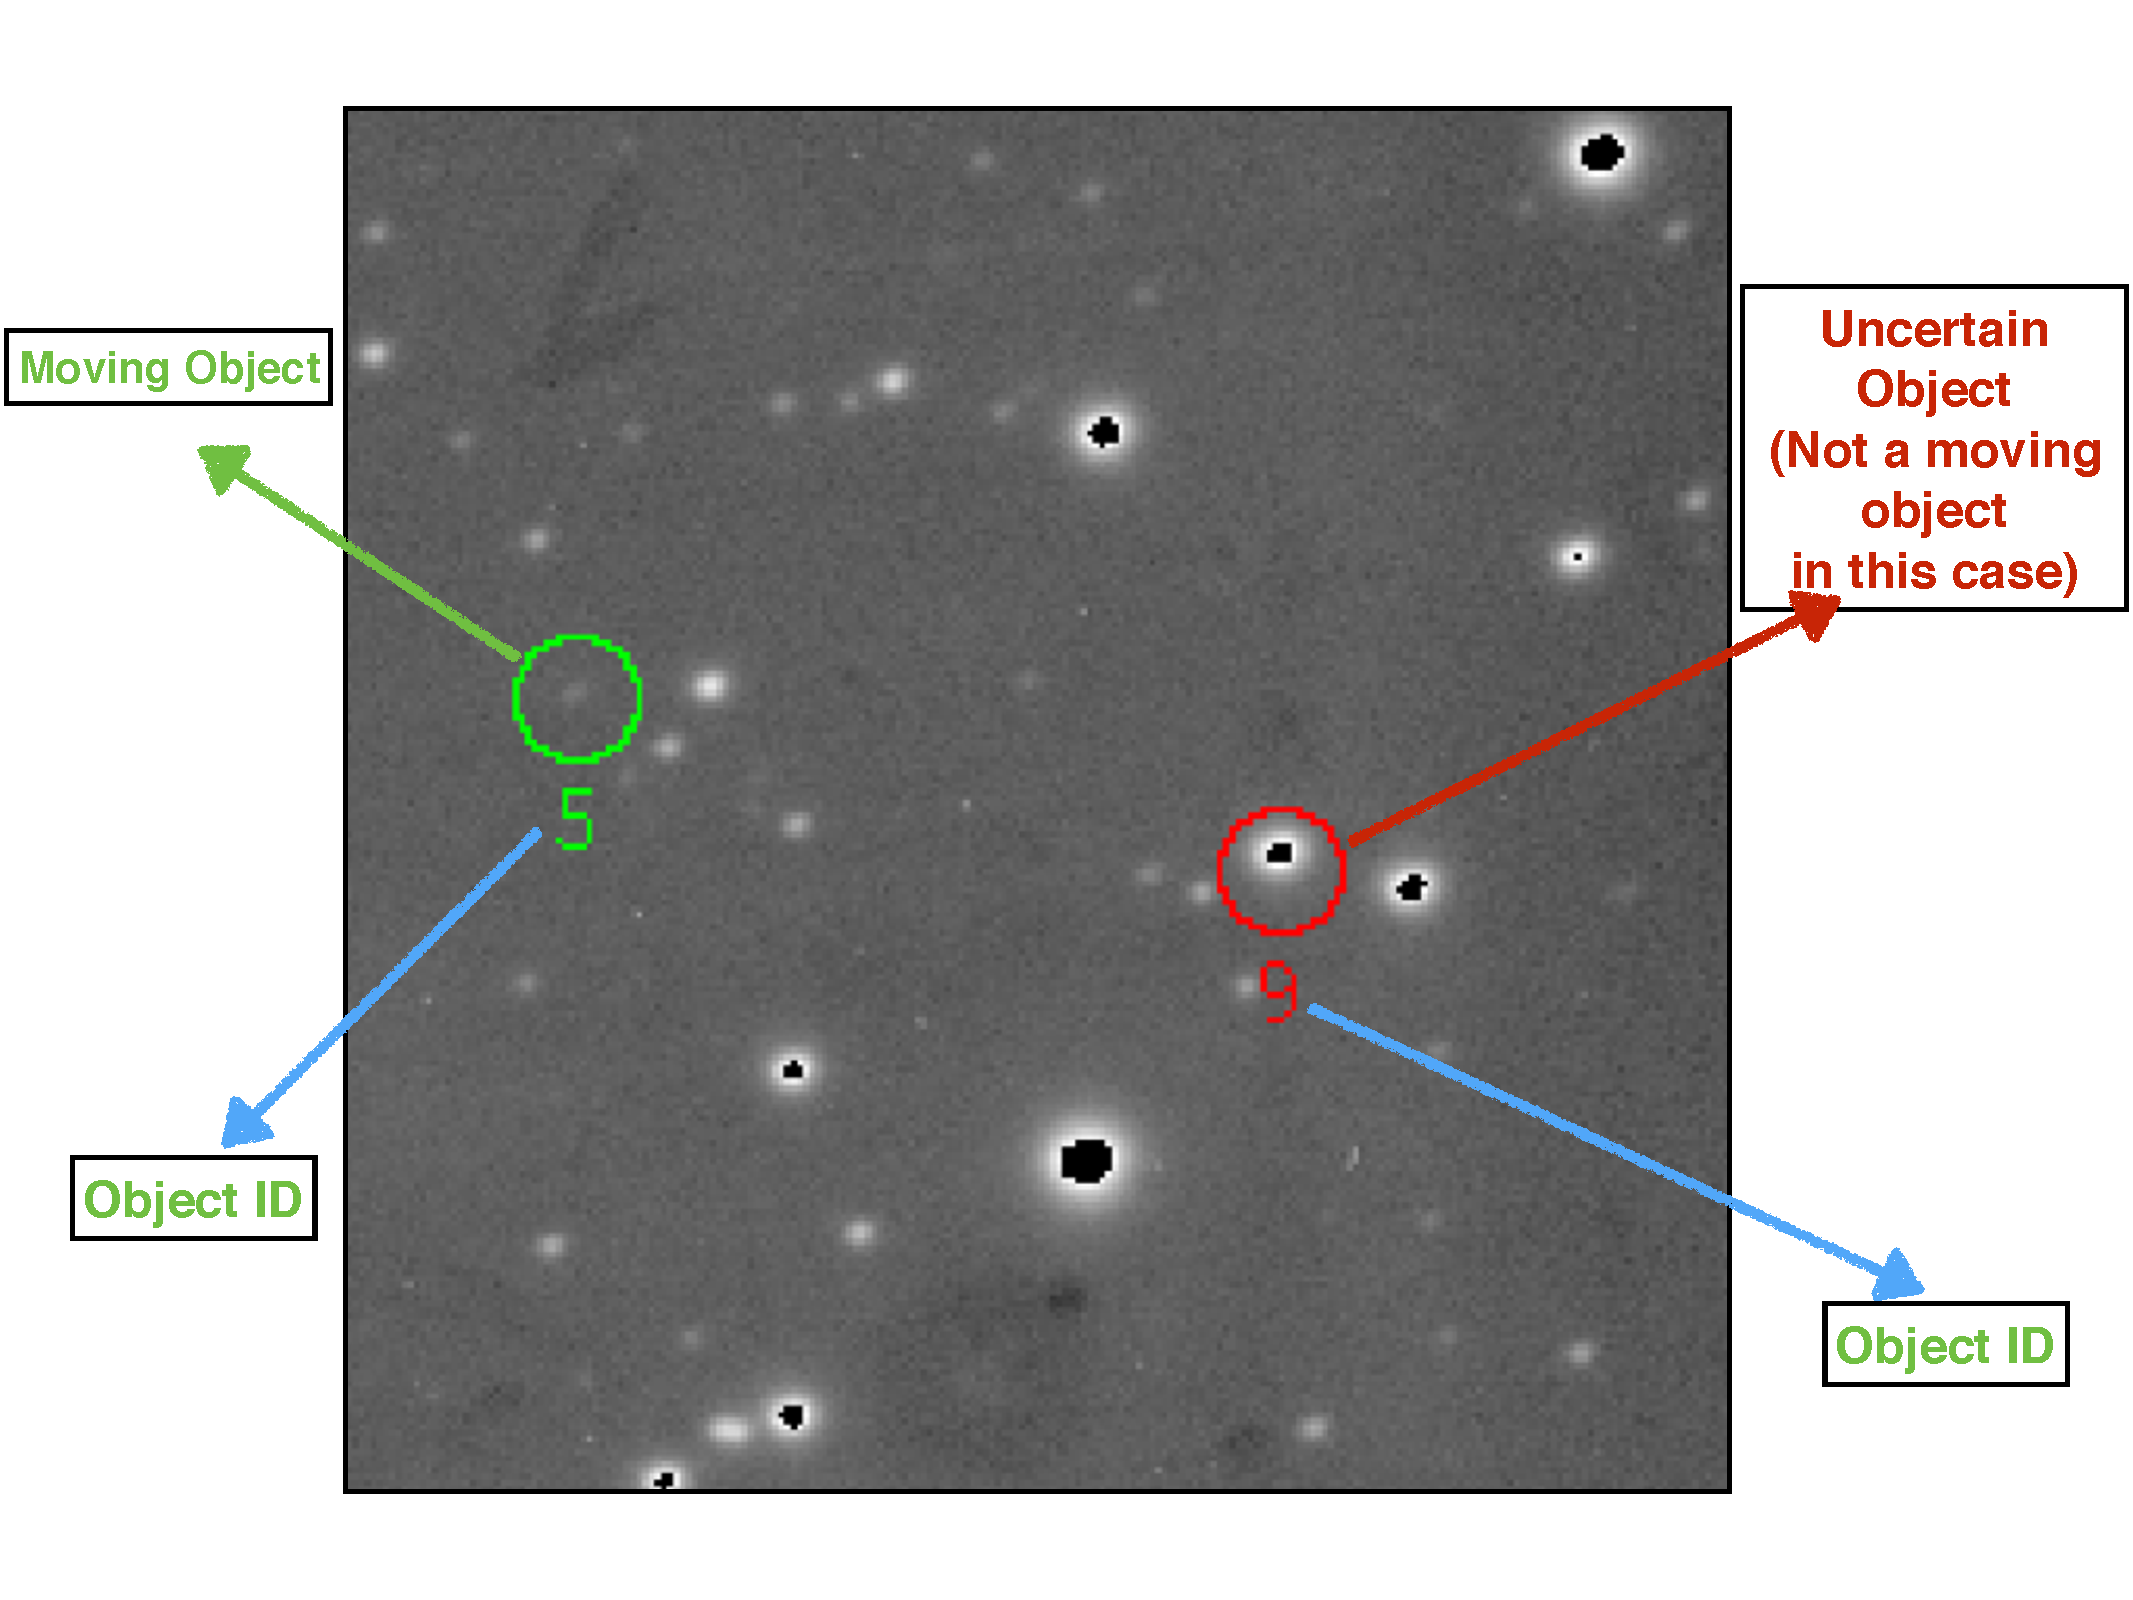
\includegraphics[width=1.0\textwidth]{figure_6_real_image}
  \caption{Part of a PNG image generated by A-Track. Green and red circles are used to mark moving and uncertain objects, respectively. Corresponding ObjectIDs are also printed using the same colors.}
  \label{fig:realimage}
\end{figure}

Finally, unless the \verb;--skip-gif; option is used in the command-line interface, an animated GIF file, named animation.gif, is created in the atrack/directory. This file shows the detected moving objects in motion.


\section{RESULTS AND DISCUSSION}

The parameters used by ILDA that affect the results most significantly are TRAVEL\_MIN, HEIGHT\_MAX, TOLERANCE, and SNR\_MIN. To test the performance effects of these parameters, we ran A-Track on two sets of sequential telescope images: 2000CA30 and Astronomia, named after the asteroids being observed. The 2000CA30 set corresponds to a dense region of the sky. The image quality is good, with more than 5000 identified sources in any image in the set. The Astronomia set was intentionally chosen to be of poor quality, with less than 400 identified sources in any image in the set. We decided that these two sets can be used to test the limits of A-Track.

The images were acquired by an SI-1100 CCD with a 1-meter telescope at TUBITAK National Observatory, Antalya, Turkey (Observatory Code: A84). We used raw images for testing (no reduction). There were 7 sequential images in each set. All images had the same XBIN and YBIN value of 2 and the same NAXIS1 and NAXIS2 value of 2048. The observation times are from 2014-­02-­05T18:31:33.85 to 2014-­02-­05T20:03:14.46 for the 2000CA30 set and from 2015-­03-­08T23:09:11.89 to 2015-­03-­08T23:23:29.55 for Astronomia. The exposure times for the images are 700-800 seconds in 2000CA30 and 80-100 seconds in Astronomia. The tests were done on a 2.6 GHz Intel®Core™ i5 3230M processor (4 virtual cores) with 2 GB 1600 MHz GDDR3 RAM running GNU/Linux Xubuntu 14.04 LTS.

The default parameters in the [Sources] section of the configuration file were used for these tests. These are the parameters recommended by Bertin to catch the faintest objects in the images \citep{sextractor_manual}. As for the four parameters being tested, we kept three of the parameters at their default values while varying the fourth one. The moving objects are tagged as True or False detections after checking the images visually. The results are given in Tables 1-4.

The results for TRAVEL\_MIN are given in Table \ref{tab:travelmin}. TRAVEL\_MIN defines the minimum distance a truly moving object has to travel between consecutive images. It can be considered as a speed filter. Its default value is 0.5 (pixels). Decreasing this value will help ILDA catch slower moving objects at the expense of an increased number of false detections, mostly because of the variations in the central coordinates of the stars due to pixel saturation or different atmospheric conditions between images. Increasing this value too much will result in fewer number of detections since only fast enough objects will be detected by ILDA.

% TRAVEL_MIN
\begin{table}[H]
    \begin{subtable}[h]{0.45\textwidth}
        \centering
        \scalebox{0.5}{
        \begin{tabular}{@{}>{\Large}c>{\Large}c>{\Large}c>{\Large}c>{\Large}c>{\Large}c@{}}
		 \toprule
                 \multicolumn{6}{c}{\Large\textbf{2000CA30}} \\ \midrule
             \small\textbf{\begin{tabular}[c]{@{}c@{}} TRAVEL\_MIN\\(px)\end{tabular}} & \small\textbf{ASTPLOT} & \small\textbf{\begin{tabular}[c]{@{}c@{}}A-Track\\TRUE\end{tabular}} & \small\textbf{\begin{tabular}[c]{@{}c@{}}A-Track\\FALSE\end{tabular}} & \small\textbf{\begin{tabular}[c]{@{}c@{}}UNCERTAIN\end{tabular}} & \small\textbf{\begin{tabular}[c]{@{}c@{}}PROCESS\\TIME (s)\end{tabular}}\\ \midrule
		 0.1 & 7 & 7 & 430 & 449 & 657 \\
		 0.2 & 7 & 7 & 2 & 45 & 92 \\
		 0.3 & 7 & 7 & 0 & 8 & 74  \\
		 0.4 & 7 & 7 & 0 & 4 & 62  \\
		 \rowcolor{LightCyan}
		 0.5 & 7 & 7 & 0 & 2 & 30 \\
		 0.6 & 7 & 7 & 0 & 2 & 29 \\
		 0.7 & 7 & 7 & 0 & 0 & 26 \\
		 0.8 & 7 & 7 & 0 & 0 & 26 \\
		 0.9 & 7 & 7 & 0 & 0 & 27 \\
		 1.00 & 7 & 7 & 0 & 0 & 27 \\
		 1.10 & 7 & 7 & 0 & 0 & 26 \\
		 1.20 & 7 & 7 & 0 & 0 & 27 \\
		 1.30 & 7 & 7 & 0 & 0 & 27 \\
		 1.40 & 7 & 7 & 0 & 0 & 26 \\
		 1.50 & 7 & 7 & 0 & 0 & 26 \\
		 1.60 & 7 & 7 & 0 & 0 & 27 \\
		 1.70 & 7 & 7 & 0 & 0 & 26 \\
		 1.80 & 7 & 7 & 0 & 0 & 27 \\
		 1.90 & 7 & 7 & 0 & 0 & 27 \\
		 2.00 & 7 & 5 & 0 & 0 & 27 \\
		 2.10 & 7 & 5 & 0 & 0 & 27 \\
		 2.20 & 7 & 5 & 0 & 0 & 29 \\
		 2.30 & 7 & 5 & 0 & 0 & 26 \\
		 2.40 & 7 & 4 & 0 & 0 & 27 \\
		 2.50 & 7 & 4 & 0 & 0 & 26 \\
		 2.60 & 7 & 3 & 0 & 0 & 27 \\
		 2.70 & 7 & 3 & 0 & 0 & 27 \\
		 2.80 & 7 & 2 & 0 & 0 & 26 \\
		 2.90 & 7 & 2 & 0 & 0 & 26 \\
		 3.00 & 7 & 2 & 0 & 0 & 26 \\
        \end{tabular}
        }
        \caption{2000CA30}
        \label{tab:2000CA30_travelmin}
    \end{subtable}
    \hfill
    \begin{subtable}[h]{0.45\textwidth}
        \centering
        \scalebox{0.5}{
        \begin{tabular}{@{}>{\Large}c>{\Large}c>{\Large}c>{\Large}c>{\Large}c>{\Large}c@{}}
		 \toprule
                 \multicolumn{6}{c}{\Large\textbf{Astronomia}} \\ \midrule
             \small\textbf{\begin{tabular}[c]{@{}c@{}} TRAVEL\_MIN\\(px)\end{tabular}} & \small\textbf{ASTPLOT} & \small\textbf{\begin{tabular}[c]{@{}c@{}}A-Track\\TRUE\end{tabular}} & \small\textbf{\begin{tabular}[c]{@{}c@{}}A-Track\\FALSE\end{tabular}} & \small\textbf{\begin{tabular}[c]{@{}c@{}}UNCERTAIN\end{tabular}} & \small\textbf{\begin{tabular}[c]{@{}c@{}}PROCESS\\TIME (s)\end{tabular}}\\ \midrule
		0.1 & 6 & 3 & 3 & 38 & 23 \\
		0.2 & 6 & 3 & 2 & 4 & 26 \\
		0.3 & 6 & 2 & 0 & 0 & 24 \\
		0.4 & 6 & 2 & 0 & 0 & 24 \\
		\rowcolor{LightCyan}
		0.5 & 6 & 2 & 0 & 0 & 24 \\
		0.6 & 6 & 2 & 0 & 0 & 24 \\
		0.7 & 6 & 2 & 0 & 0 & 24 \\
		0.8 & 6 & 2 & 0 & 0 & 24 \\
		0.9 & 6 & 2 & 0 & 0 & 24 \\
		1.00 & 6 & 2 & 0 & 0 & 24 \\
		1.10 & 6 & 2 & 0 & 0 & 24 \\
		1.20 & 6 & 2 & 0 & 0 & 24 \\
		1.30 & 6 & 1 & 0 & 0 & 24 \\
		1.40 & 6 & 1 & 0 & 0 & 24 \\
		1.50 & 6 & 1 & 0 & 0 & 24 \\
		1.60 & 6 & 1 & 0 & 0 & 26 \\
		1.70 & 6 & 0 & 0 & 0 & 10 \\
		1.80 & 6 & 0 & 0 & 0 & 10 \\
		1.90 & 6 & 0 & 0 & 0 & 10 \\
		2.00 & 6 & 0 & 0 & 0 & 10 \\
		2.10 & 6 & 0 & 0 & 0 & 10 \\
		2.20 & 6 & 0 & 0 & 0 & 10 \\
		2.30 & 6 & 0 & 0 & 0 & 10 \\
		2.40 & 6 & 0 & 0 & 0 & 10 \\
		2.50 & 6 & 0 & 0 & 0 & 10 \\
		2.60 & 6 & 0 & 0 & 0 & 10 \\
		2.70 & 6 & 0 & 0 & 0 & 10 \\
		2.80 & 6 & 0 & 0 & 0 & 10 \\
		2.90 & 6 & 0 & 0 & 0 & 10 \\
		3.00 & 6 & 0 & 0 & 0 & 10 \\
        \end{tabular}
        }
        \caption{Astronomia}
        \label{tab:astronomia_travelmin}
    \end{subtable}
    \caption{A-Track results for the data sets 2000CA30 and Astronomia for different values of the TRAVEL\_MIN parameter. The row that corresponds to the default value of 0.5 is highlighted. The actual number of moving objects reported by ASTPLOT, the number of true detections by A-Track, the number of false detections by A-Track, the number of uncertain objects found by A-Track, and the processing time are shown in respective columns.}
    \label{tab:travelmin}
\end{table}

The results for HEIGHT\_MAX are given in Table \ref{tab:heightmax}. HEIGHT\_MAX defines the maximum height a 3-point combination can have in order to be considered as collinear (Fig.~\ref{fig:linesegment}). Its default value is 0.1 (pixels). Increasing this value will help ILDA catch more moving objects at the expense of an increased number of false/uncertain detections. Again, this is due to the small variations in the central coordinates of the objects identified by SExtractor.

% HEIGHT_MAX
\begin{table}[H]
    \begin{subtable}[h]{0.45\textwidth}
        \centering
        \scalebox{0.5}{
        \begin{tabular}{@{}>{\Large}c>{\Large}c>{\Large}c>{\Large}c>{\Large}c>{\Large}c@{}}
		 \toprule
		 \multicolumn{6}{c}{\Large\textbf{2000CA30}} \\ \midrule
             \small\textbf{\begin{tabular}[c]{@{}c@{}} HEIGHT\_MAX\\(px)\end{tabular}} & \small\textbf{ASTPLOT} & \small\textbf{\begin{tabular}[c]{@{}c@{}}A-Track\\TRUE\end{tabular}} & \small\textbf{\begin{tabular}[c]{@{}c@{}}A-Track\\FALSE\end{tabular}} & \small\textbf{\begin{tabular}[c]{@{}c@{}}UNCERTAIN\end{tabular}} & \small\textbf{\begin{tabular}[c]{@{}c@{}}PROCESS\\TIME (s)\end{tabular}}\\ \midrule
			0.05 & 7 & 6 & 0 & 4 & 69 \\
			\rowcolor{LightCyan}
			0.10 & 7 & 7 & 0 & 6 & 67 \\
			0.15 & 7 & 7 & 1 & 11 & 66 \\
			0.20 & 7 & 7 & 1 & 12 & 70 \\
			0.25 & 7 & 7 & 2 & 16 & 70 \\
			0.30 & 7 & 7 & 2 & 17 & 78 \\
			0.35 & 7 & 7 & 2 & 19 & 76 \\
			0.40 & 7 & 7 & 3 & 21 & 79 \\
			0.45 & 7 & 7 & 4 & 27 & 78 \\
			0.50 & 7 & 7 & 4 & 28 & 78 \\
			0.55 & 7 & 7 & 4 & 28 & 66 \\
			0.60 & 7 & 7 & 4 & 28 & 68 \\
			0.65 & 7 & 7 & 4 & 29 & 65 \\
			0.70 & 7 & 7 & 6 & 27 & 67 \\
			0.75 & 7 & 7 & 6 & 28 & 67 \\
			0.80 & 7 & 7 & 6 & 28 & 70 \\
			0.85 & 7 & 7 & 7 & 29 & 70 \\
			0.90 & 7 & 7 & 8 & 28 & 68 \\
			0.95 & 7 & 7 & 9 & 29 & 66 \\
			1.00 & 7 & 7 & 9 & 29 & 66 \\
        \end{tabular}
        }
        \caption{2000CA30}
        \label{tab:2000CA30_hmax}
    \end{subtable}
    \hfill
    \begin{subtable}[h]{0.45\textwidth}
        \centering
        \scalebox{0.5}{
        \begin{tabular}{@{}>{\Large}c>{\Large}c>{\Large}c>{\Large}c>{\Large}c>{\Large}c@{}}
		 \toprule
		 \multicolumn{6}{c}{\Large\textbf{Astronomia}} \\ \midrule
             \small\textbf{\begin{tabular}[c]{@{}c@{}} HEIGHT\_MAX\\(px)\end{tabular}} & \small\textbf{ASTPLOT} & \small\textbf{\begin{tabular}[c]{@{}c@{}}A-Track\\TRUE\end{tabular}} & \small\textbf{\begin{tabular}[c]{@{}c@{}}A-Track\\FALSE\end{tabular}} & \small\textbf{\begin{tabular}[c]{@{}c@{}}UNCERTAIN\end{tabular}} & \small\textbf{\begin{tabular}[c]{@{}c@{}}PROCESS\\TIME (s)\end{tabular}}\\ \midrule
			0.05 & 6 & 2 & 0 & 0 & 24 \\
			\rowcolor{LightCyan}
			0.10 & 6 & 2 & 0 & 0 & 24 \\
			0.15 & 6 & 2 & 0 & 0 & 24 \\
			0.20 & 6 & 2 & 0 & 0 & 24 \\
			0.25 & 6 & 2 & 0 & 0 & 24 \\
			0.30 & 6 & 2 & 0 & 2 & 24 \\
			0.35 & 6 & 2 & 0 & 2 & 24 \\
			0.40 & 6 & 2 & 0 & 2 & 24 \\
			0.45 & 6 & 2 & 0 & 3 & 24 \\
			0.50 & 6 & 2 & 0 & 3 & 24 \\
			0.55 & 6 & 2 & 0 & 3 & 24 \\
			0.60 & 6 & 3 & 0 & 3 & 24 \\
			0.65 & 6 & 3 & 0 & 3 & 24 \\
			0.70 & 6 & 3 & 0 & 3 & 25 \\
			0.75 & 6 & 3 & 0 & 3 & 24 \\
			0.80 & 6 & 3 & 0 & 3 & 24 \\
			0.85 & 6 & 3 & 0 & 3 & 24 \\
			0.90 & 6 & 3 & 0 & 3 & 21 \\
			0.95 & 6 & 3 & 0 & 3 & 24 \\
			1.00 & 6 & 3 & 0 & 3 & 24 \\
        \end{tabular}
        }
        \caption{Astronomia}
        \label{tab:astronomia_hmax}
    \end{subtable}
    \caption{A-Track results for the data sets 2000CA30 and Astronomia for different values of the HEIGHT\_MAX parameter. The row that corresponds to the default value of 0.1 is highlighted. The actual number of moving objects reported by ASTPLOT, the number of true detections by A-Track, the number of false detections by A-Track, the number of uncertain objects found by A-Track, and the processing time are shown in respective columns.}
    \label{tab:heightmax}
\end{table}

The results for TOLERANCE are given in Table \ref{tab:tau}. TOLERANCE defines the tolerable spatial shift of the third point during the speed check. Its default value is 1.0 (pixels). Assuming the time information in the FITS-headers are correct, there is no need to increase this value. Increasing this value will result in an increased number of false and uncertain detections.

% TOLERANCE
\begin{table}[H]
    \begin{subtable}[h]{0.45\textwidth}
        \centering
        \scalebox{0.5}{
        \begin{tabular}{@{}>{\Large}c>{\Large}c>{\Large}c>{\Large}c>{\Large}c>{\Large}c@{}}
		 \toprule
		 \multicolumn{6}{c}{\Large\textbf{2000CA30}} \\ \midrule
             \small\textbf{\begin{tabular}[c]{@{}c@{}} TOLERANCE\\(px)\end{tabular}} & \small\textbf{ASTPLOT} & \small\textbf{\begin{tabular}[c]{@{}c@{}}A-Track\\TRUE\end{tabular}} & \small\textbf{\begin{tabular}[c]{@{}c@{}}A-Track\\FALSE\end{tabular}} & \small\textbf{\begin{tabular}[c]{@{}c@{}}UNCERTAIN\end{tabular}} & \small\textbf{\begin{tabular}[c]{@{}c@{}}PROCESS\\TIME (s)\end{tabular}}\\ \midrule
		 0.25 & 7 & 7 & 0 & 2 & 73 \\
		 0.50 & 7 & 7 & 0 & 4 & 71 \\
		 0.75 & 7 & 7 & 0 & 6 & 72 \\
		 \rowcolor{LightCyan}
		 1.00 & 7 & 7 & 0 & 6 & 71 \\
		 1.25 & 7 & 7 & 1 & 8 & 73 \\
		 1.50 & 7 & 7 & 1 & 9 & 73 \\
		 1.75 & 7 & 7 & 1 & 11 & 70 \\
		 2.00 & 7 & 7 & 2 & 11 & 74 \\
		 2.25 & 7 & 7 & 2 & 13 & 75 \\
		 2.50 & 7 & 7 & 2 & 13 & 72 \\
		 2.75 & 7 & 7 & 2 & 15 & 74 \\
		 3.00 & 7 & 7 & 2 & 14 & 74 \\
		 3.25 & 7 & 7 & 3 & 14 & 72 \\
		 3.50 & 7 & 7 & 4 & 12 & 75 \\
		 3.75 & 7 & 7 & 4 & 13 & 72 \\
		 4.00 & 7 & 7 & 4 & 14 & 75
        \end{tabular}
        }
        \caption{2000CA30}
        \label{tab:2000CA30_tolerance}
    \end{subtable}
    \hfill
    \begin{subtable}[h]{0.45\textwidth}
        \centering
        \scalebox{0.5}{
        \begin{tabular}{@{}>{\Large}c>{\Large}c>{\Large}c>{\Large}c>{\Large}c>{\Large}c@{}}
		 \toprule
		 \multicolumn{6}{c}{\Large\textbf{Astronomia}} \\ \midrule
             \small\textbf{\begin{tabular}[c]{@{}c@{}} TOLERANCE\\(px)\end{tabular}} & \small\textbf{ASTPLOT} & \small\textbf{\begin{tabular}[c]{@{}c@{}}A-Track\\TRUE\end{tabular}} & \small\textbf{\begin{tabular}[c]{@{}c@{}}A-Track\\FALSE\end{tabular}} & \small\textbf{\begin{tabular}[c]{@{}c@{}}UNCERTAIN\end{tabular}} & \small\textbf{\begin{tabular}[c]{@{}c@{}}PROCESS\\TIME (s)\end{tabular}}\\ \midrule
		 0.25 & 6 & 2 & 0 & 0 & 25 \\
		 0.50 & 6 & 2 & 0 & 0 & 24 \\
		 0.75 & 6 & 2 & 0 & 0 & 24 \\
		 \rowcolor{LightCyan}
		 1.00 & 6 & 2 & 0 & 0 & 24 \\
		 1.25 & 6 & 2 & 0 & 0 & 24 \\
		 1.50 & 6 & 2 & 0 & 0 & 24 \\
		 1.75 & 6 & 2 & 0 & 0 & 24 \\
		 2.00 & 6 & 2 & 0 & 0 & 24 \\
		 2.25 & 6 & 2 & 0 & 0 & 25 \\
		 2.50 & 6 & 2 & 0 & 0 & 25 \\
		 2.75 & 6 & 2 & 0 & 0 & 24 \\
		 3.00 & 6 & 2 & 0 & 0 & 24 \\
		 3.25 & 6 & 2 & 0 & 0 & 24 \\
		 3.50 & 6 & 2 & 0 & 0 & 25 \\
		 3.75 & 6 & 2 & 0 & 0 & 24 \\
		 4.00 & 6 & 2 & 0 & 0 & 24
        \end{tabular}
        }
        \caption{Astronomia}
        \label{tab:astronomia_tolerance}
    \end{subtable}
    \caption{A-Track results for the data sets 2000CA30 and Astronomia for different values of the TOLERANCE parameter. The row that corresponds to the default value of 1 is highlighted. The actual number of moving objects reported by ASTPLOT, the number of true detections by A-Track, the number of false detections by A-Track, the number of uncertain objects found by A-Track, and the processing time are shown in respective columns.}
    \label{tab:tau}
\end{table}

The results for SNR\_MIN are given in Table \ref{tab:snr}. SNR\_MIN defines the minimum signal-to-noise ratio for a moving object. Its default value is 10. Increasing this value will reduce the processing time at the expense of fainter moving objects going undetected.

% SNR_MIN
\begin{table}[H]
    \begin{subtable}[h]{0.45\textwidth}
        \centering
        \scalebox{0.5}{
        \begin{tabular}{@{}>{\Large}c>{\Large}c>{\Large}c>{\Large}c>{\Large}c>{\Large}c@{}}
		 \toprule
		 \multicolumn{6}{c}{\Large\textbf{2000CA30}} \\ \midrule
             \small\textbf{SNR\_MIN} & \small\textbf{ASTPLOT} & \small\textbf{\begin{tabular}[c]{@{}c@{}}A-Track\\TRUE\end{tabular}} & \small\textbf{\begin{tabular}[c]{@{}c@{}}A-Track\\FALSE\end{tabular}} & \small\textbf{\begin{tabular}[c]{@{}c@{}}UNCERTAIN\end{tabular}} & \small\textbf{\begin{tabular}[c]{@{}c@{}}PROCESS\\TIME (s)\end{tabular}}\\ \midrule
		 2.5 & 7 & 7 & 0 & 6 & 71 \\
		 5 & 7 & 7 & 0 & 6 & 64 \\
		 7.5 & 7 & 7 & 0 & 6 & 71 \\
		 \rowcolor{LightCyan}
		 10 & 7 & 7 & 0 & 6 & 64 \\
		 12.5 & 7 & 6 & 0 & 6 & 71 \\
		 15 & 7 & 5 & 0 & 6 & 62 \\
		 17.5 & 7 & 5 & 0 & 6 & 69 \\
		 20 & 7 & 4 & 0 & 6 & 30 \\
		 22.5 & 7 & 3 & 0 & 6 & 25 \\
		 25 & 7 & 3 & 0 & 5 & 25 \\
		 27.5 & 7 & 3 & 0 & 5 & 23 \\
		 30 & 7 & 2 & 0 & 6 & 23 \\
		 32.5 & 7 & 2 & 0 & 6 & 22 \\
		 35 & 7 & 2 & 0 & 6 & 21 \\
		 37.5 & 7 & 2 & 0 & 5 & 20 \\
		 40 & 7 & 2 & 0 & 5 & 23 \\

        \end{tabular}
        }
        \caption{2000CA30}
        \label{tab:2000CA30_snr}
    \end{subtable}
    \hfill
    \begin{subtable}[h]{0.45\textwidth}
        \centering
        \scalebox{0.5}{
        \begin{tabular}{@{}>{\Large}c>{\Large}c>{\Large}c>{\Large}c>{\Large}c>{\Large}c@{}}
		 \toprule
		 \multicolumn{6}{c}{\Large\textbf{Astronomia}} \\ \midrule
             \small\textbf{SNR\_MIN} & \small\textbf{ASTPLOT} & \small\textbf{\begin{tabular}[c]{@{}c@{}}A-Track\\TRUE\end{tabular}} & \small\textbf{\begin{tabular}[c]{@{}c@{}}A-Track\\FALSE\end{tabular}} & \small\textbf{\begin{tabular}[c]{@{}c@{}}UNCERTAIN\end{tabular}} & \small\textbf{\begin{tabular}[c]{@{}c@{}}PROCESS\\TIME (s)\end{tabular}}\\ \midrule
		 2.5 & 6 & 2 & 0 & 0 & 24 \\
		 5 & 6 & 2 & 0 & 0 & 23 \\
		 7.5 & 6 & 2 & 0 & 0 & 24 \\
		 \rowcolor{LightCyan}
		 10 & 6 & 2 & 0 & 0 & 24 \\
		 12.5 & 6 & 2 & 0 & 0 & 24 \\
		 15 & 6 & 2 & 0 & 0 & 24 \\
		 17.5 & 6 & 2 & 0 & 0 & 23 \\
		 20 & 6 & 2 & 0 & 0 & 23 \\
		 22.5 & 6 & 2 & 0 & 0 & 23 \\
		 25 & 6 & 2 & 0 & 0 & 23 \\
		 27.5 & 6 & 2 & 0 & 0 & 23 \\
		 30 & 6 & 2 & 0 & 0 & 27 \\
		 32.5 & 6 & 2 & 0 & 0 & 25 \\
		 35 & 6 & 2 & 0 & 0 & 26 \\
		 37.5 & 6 & 2 & 0 & 0 & 25 \\
		 40 & 6 & 2 & 0 & 0 & 25 \\
        \end{tabular}
        }
        \caption{Astronomia}
        \label{tab:astronomia_snr}
    \end{subtable}
    \caption{A-Track results for the data sets 2000CA30 and Astronomia for different values of the SNR\_MIN parameter. The row that corresponds to the default value of 10 is highlighted. The actual number of moving objects reported by ASTPLOT, the number of true detections by A-Track, the number of false detections by A-Track, the number of uncertain objects found by A-Track, and the processing time are shown in respective columns.}
    \label{tab:snr}
\end{table}

Information about the positions of the moving objects within the observed regions can be found at the ASTPLOT website \citep{astplot}. According to ASTPLOT, there were 7 asteroids in our 2000CA30 set at the time of observation. Using its default values, A-Track was able to detect all of them. As for the Astronomia set, ASTPLOT says 6 asteroids may be seen at the time of observation. Using its default values, A-Track could detect 2 of them. As seen in Tables \ref{tab:travelmin} and \ref{tab:heightmax}, it can detect the third asteroid, which is a very slow one, if the parameters TRAVEL\_MIN or HEIGHT\_MAX are relaxed by a small factor. The remaining 3 asteroids reported by ASTPLOT are so faint that they are below the background level in our images. SExtractor cannot identify them with the recommended default parameters. We found that it is possible to detect 2 of them by decreasing the values of DETECT\_THRESH and ANALYSIS\_THRESH in the [sources] section of the configuration file. But tens of false or uncertain detections will occur in that case.

We note that the number of detectable objects depends on the overall image quality and may vary between observations. The performance of A-Track is limited by that of SExtractor, which, in turn, is affected by the atmospheric conditions at the time of observation and the condition of the telescope/CCD system used.


\section{CONCLUSION}

A-Track is a fast and efficient pipeline that uses an improved line detection algorithm (ILDA) to detect the moving objects (asteroids and comets) in sequential telescope images. It can be used to track or confirm known asteroids and comets or to discover new ones. Occasionally, moving objects that are supposed to be within the observed region will not appear in the acquired images due to very low brightness, poor telescope/CCD conditions, or atmospheric effects. A-Track will detect any moving object provided that the object is caught by the telescope/CCD system and identified by SExtractor. Since A-Track doesn't need human interaction while running, we believe it'll become a useful tool for both professional and amateur observers.

A-Track is still under development. Currently, we are working on automating the World Coordinate System (WCS) transformations of the detected moving objects. We plan on adding an automatic reporting (to Minor Planet Center) functionality as well as a user-friendly GUI to our pipeline in the future.


\section*{ACKNOWLEDGMENT}

This work was supported by The Scientific and Technological Research Council of Turkey (TUBITAK), Project Number 114F477. We would also like to thank TUBITAK for their partial support in using the T100 telescope under project number 14BT100-648.

\section*{References}

\bibliography{atrack}

\end{document}
